\section{CP and Scheduling Literature Survey}

\begin{frame}
\frametitle{A Survey of the Existing Literature}
\begin{itemize}
\item Joint work with Cemalettin Öztürk, MTU
\item What is out there
\item Where to start
\item Where to publish
\item I'm interested in some specific topic, what is relevant
\end{itemize}
\end{frame}

\begin{frame}
\frametitle{Methodology}
\begin{itemize}
\item Manually curated list of works, somewhat inclusive
\item Starting with bibtex files
\item Citation links through \href{https://opencitations.net/}{OpenCitations} (open access)
\item Content analysis on local copies of pdf files
\item Closure of domain by analyzing missing cited and citing works 
\item Limited manual analysis of works (datasets, code)
\item Results presented as LaTeX documents
\item Open source analysis on git: \url{https://hsimonis.github.io/pthg24/}
\end{itemize}
\end{frame}

\begin{frame}
\frametitle{Overall Analysis (Based on 671 Works)}
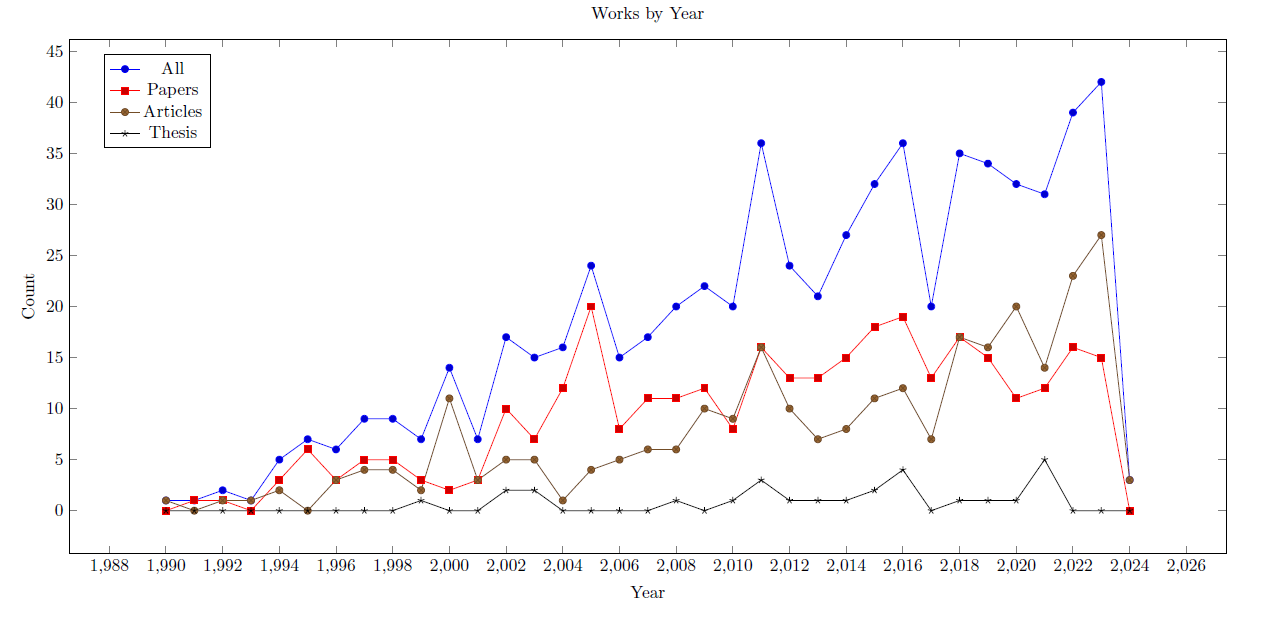
\includegraphics[width=\textwidth]{survey/worksbyyear}
\end{frame}

\begin{frame}
\frametitle{Origin of Papers/Articles}
\begin{tabular}[t]{cc}
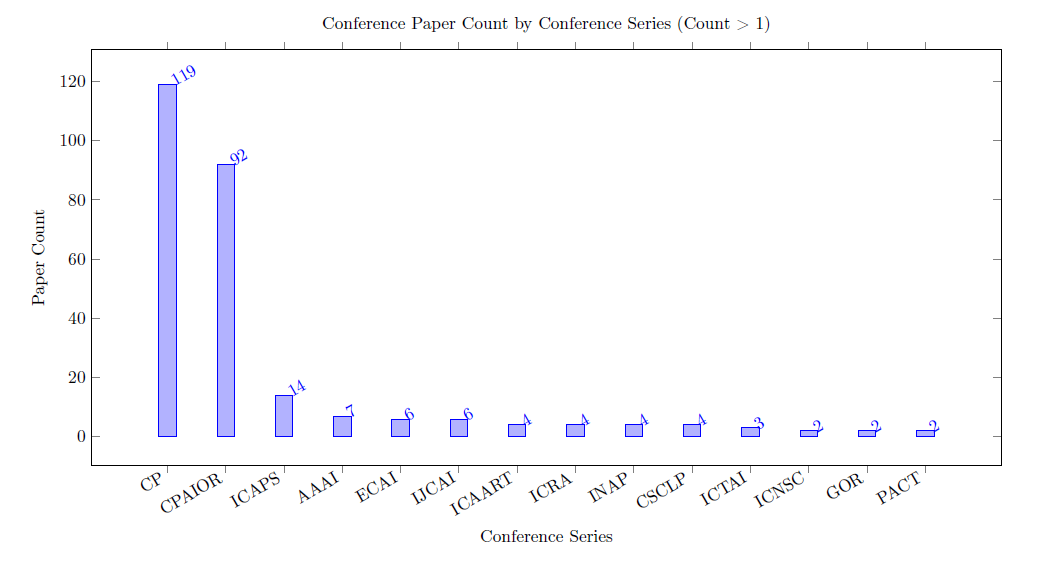
\includegraphics[width=.45\textwidth]{survey/conferences}
& 
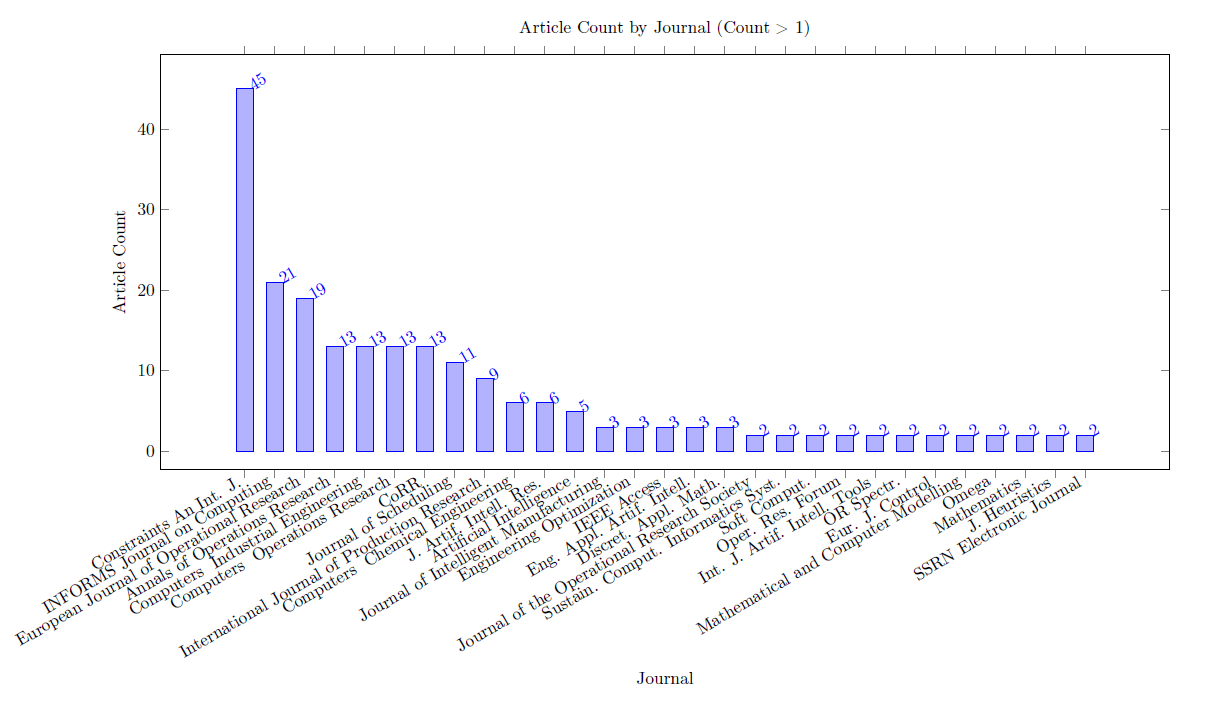
\includegraphics[width=.55\textwidth]{survey/journals}
\end{tabular}
\end{frame}

\begin{frame}
\frametitle{Most Recent Articles}
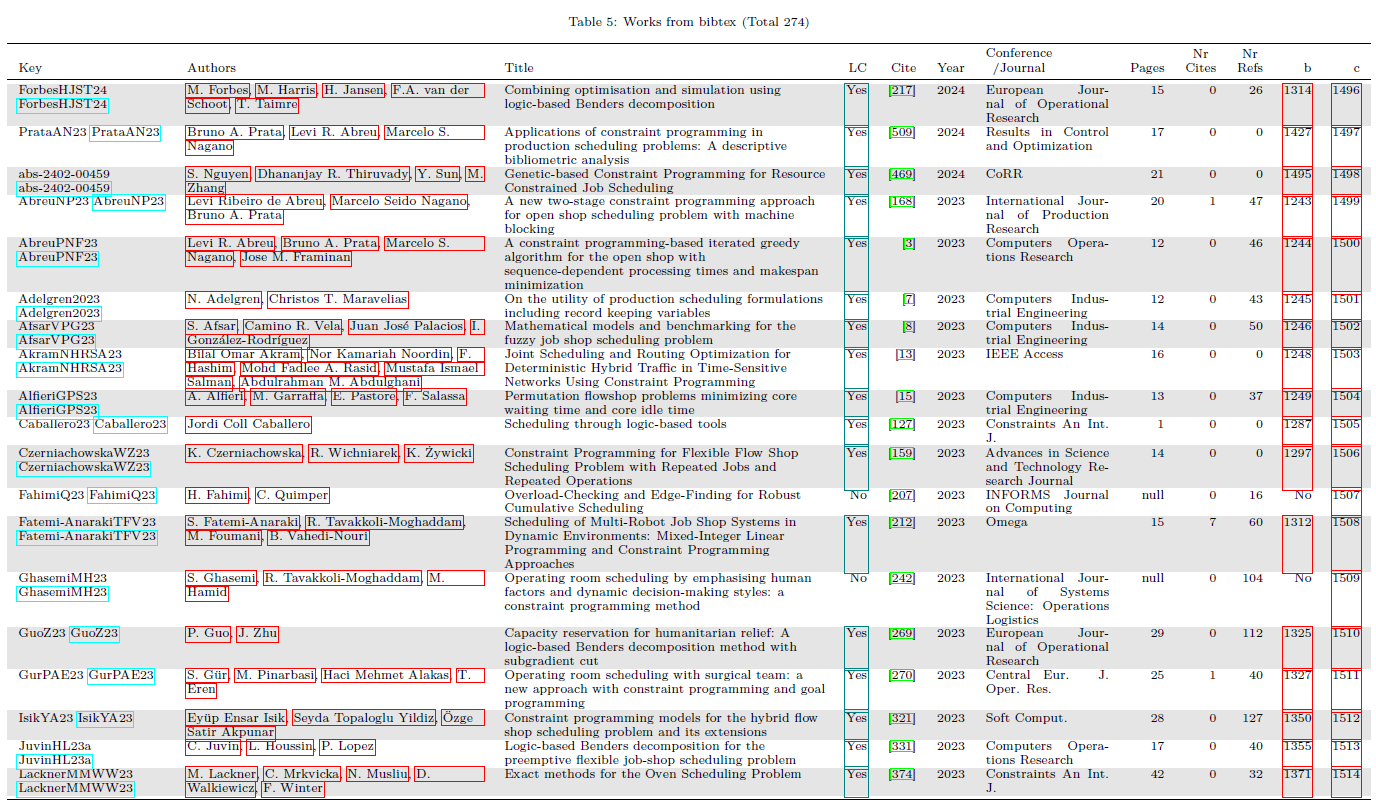
\includegraphics[width=\textwidth]{survey/mostrecentarticles}
\end{frame}

\begin{frame}
\frametitle{Automatically Extracted Article Features}
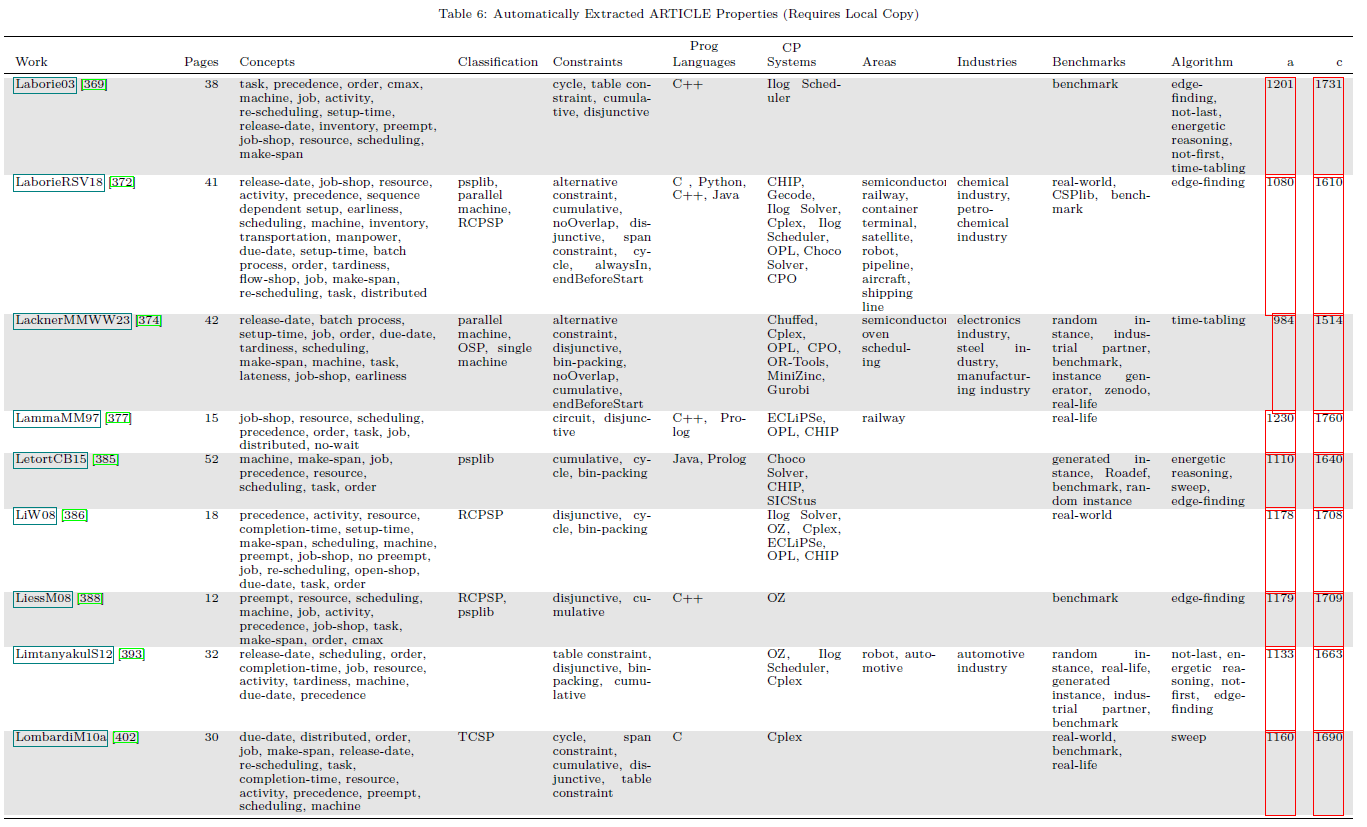
\includegraphics[width=\textwidth]{survey/extracted}
\end{frame}

\begin{frame}
\frametitle{Manually Extracted Article Features}
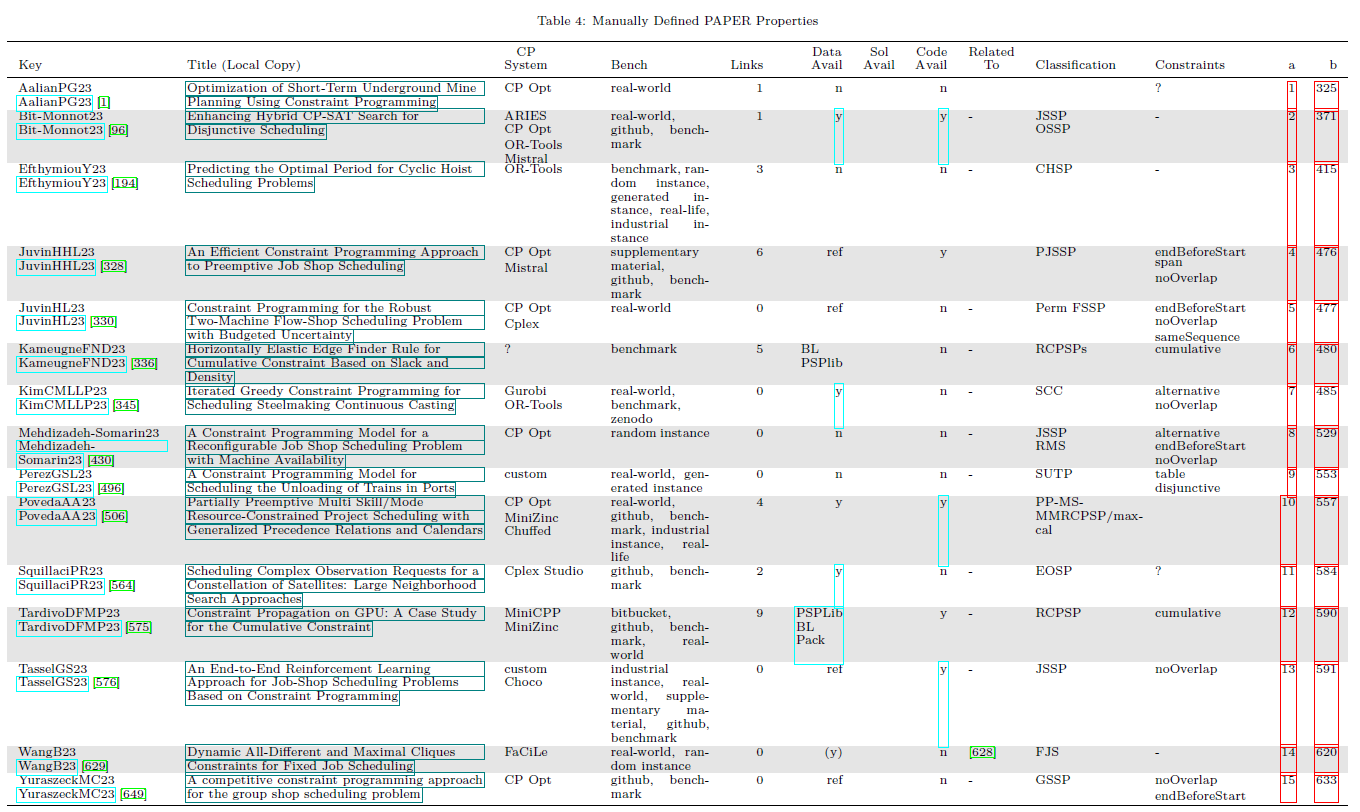
\includegraphics[width=\textwidth]{survey/manual}
\end{frame}


\begin{frame}
\frametitle{Extracted Features: Application Areas}
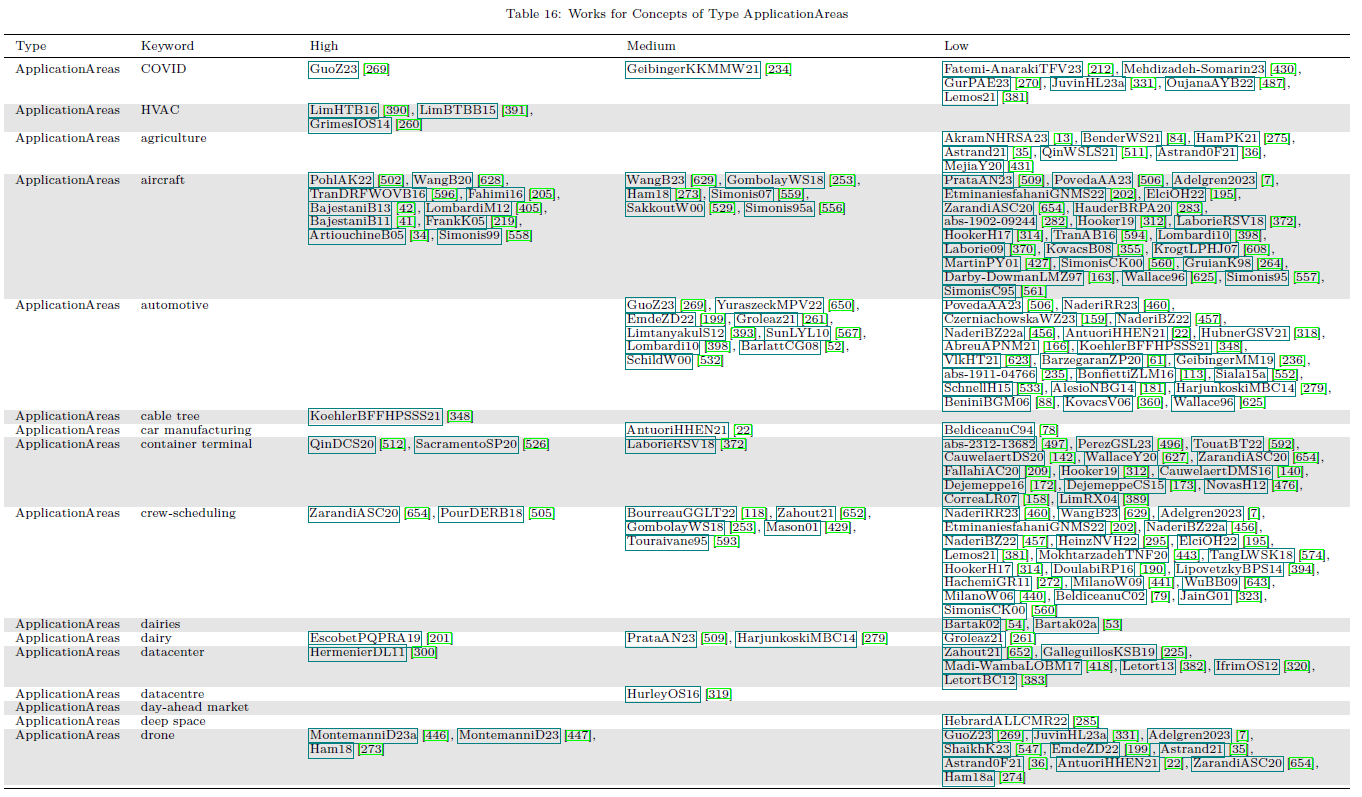
\includegraphics[width=\textwidth]{survey/applicationareas}
\end{frame}

\begin{frame}
\frametitle{Prolific Authors}
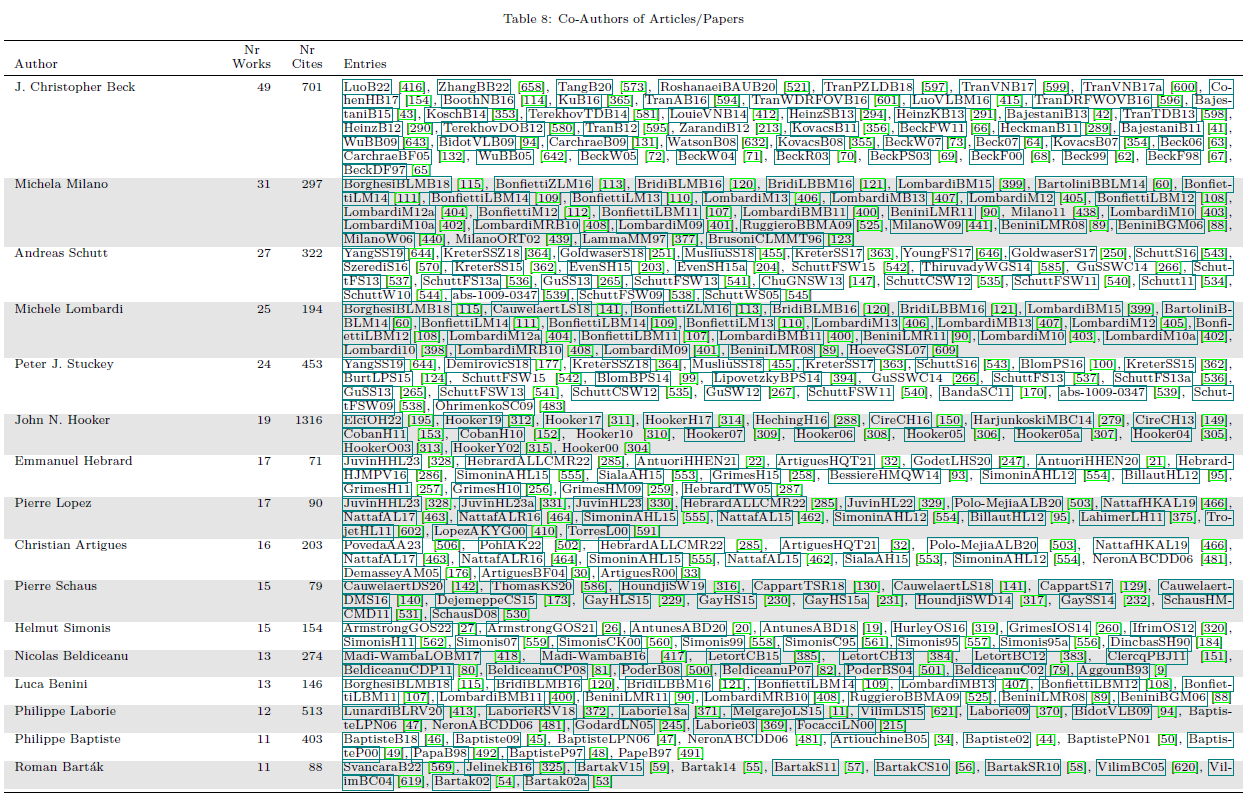
\includegraphics[width=\textwidth]{survey/authors}
\end{frame}


\begin{frame}
\frametitle{Limitations}
\begin{itemize}
\item Limited coverage by \href{https://opencitations.net/}{OpenCitations}
\item Difficult to have local access to some publication types (book, incollection)
\item Heavily biased towards publications in English
\item More powerful NLP analysis of works possible?
\end{itemize}
\end{frame}

\begin{frame}
\frametitle{Problem: Count for Most Cited Papers}
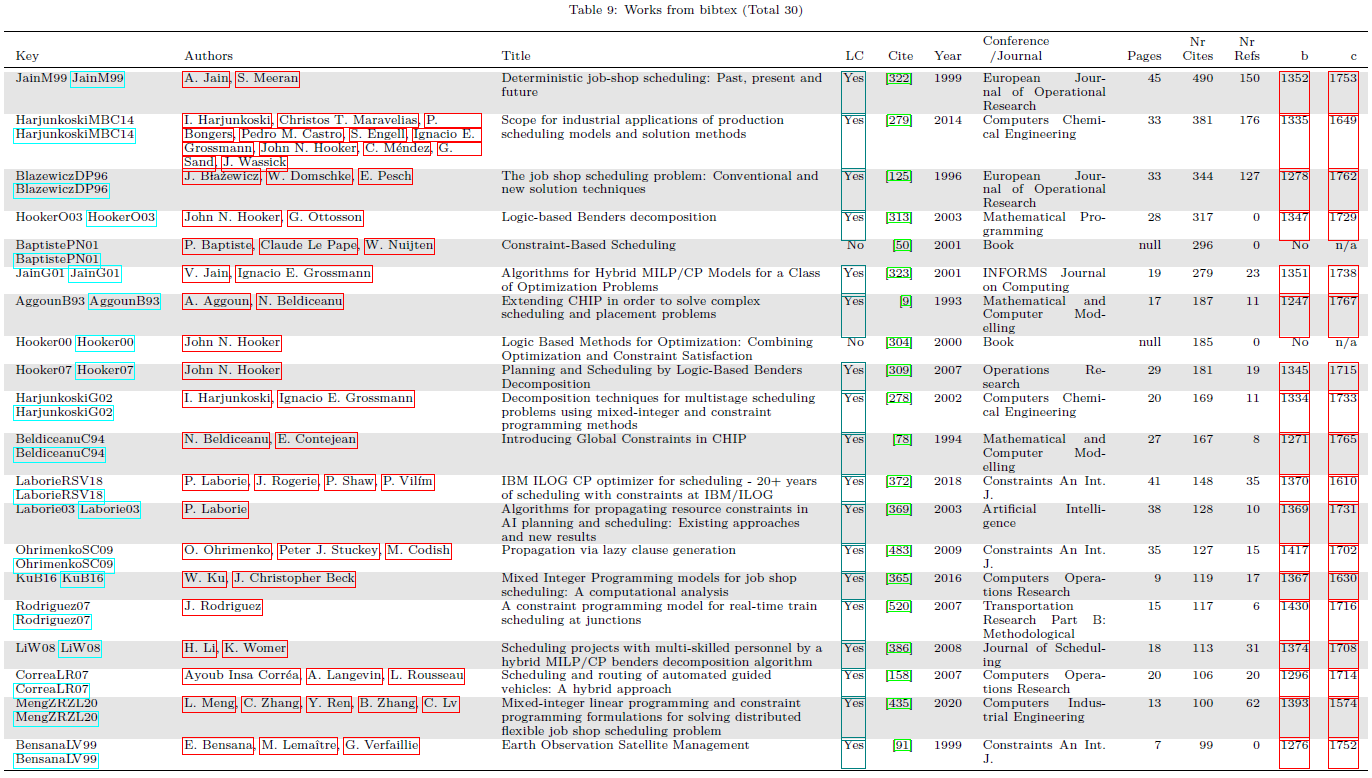
\includegraphics[width=\textwidth]{survey/mostcited}
\end{frame} 

\begin{frame}
\frametitle{OpenCitation Count Compared to Google Scholar}
\begin{tabular}{llrrr}\toprule
Key & Type & Google & OC & Ratio \\ \midrule
JainM99          & article & 1116 & 490 & 2.28\\
HarjunkoskiMBC14 & article &  588 & 381 & 1.54\\
BlazewiczDP96    & article &  796 & 344 & 2.31\\
BaptistePN01     & book    & 1039 & 296 & 3.51\\
AggounB93        & article &  502 & 187 & 2.68\\
LaborieRSV18     & article &  309 & 148 & 2.09\\
BensanaLV99      & article &  251 &  99 & 2.54\\
DincbasSH90      & article &  271 &  86 & 3.15\\
Thorsteinsson01  & paper   &  205 &  67 & 3.06\\
\midrule
DincbasSH88      & paper   &  287 &   0 & \frownie{}\\
\bottomrule
\end{tabular}
\end{frame}
 


\begin{frame}
\frametitle{Problem: Citation Count Distribution}
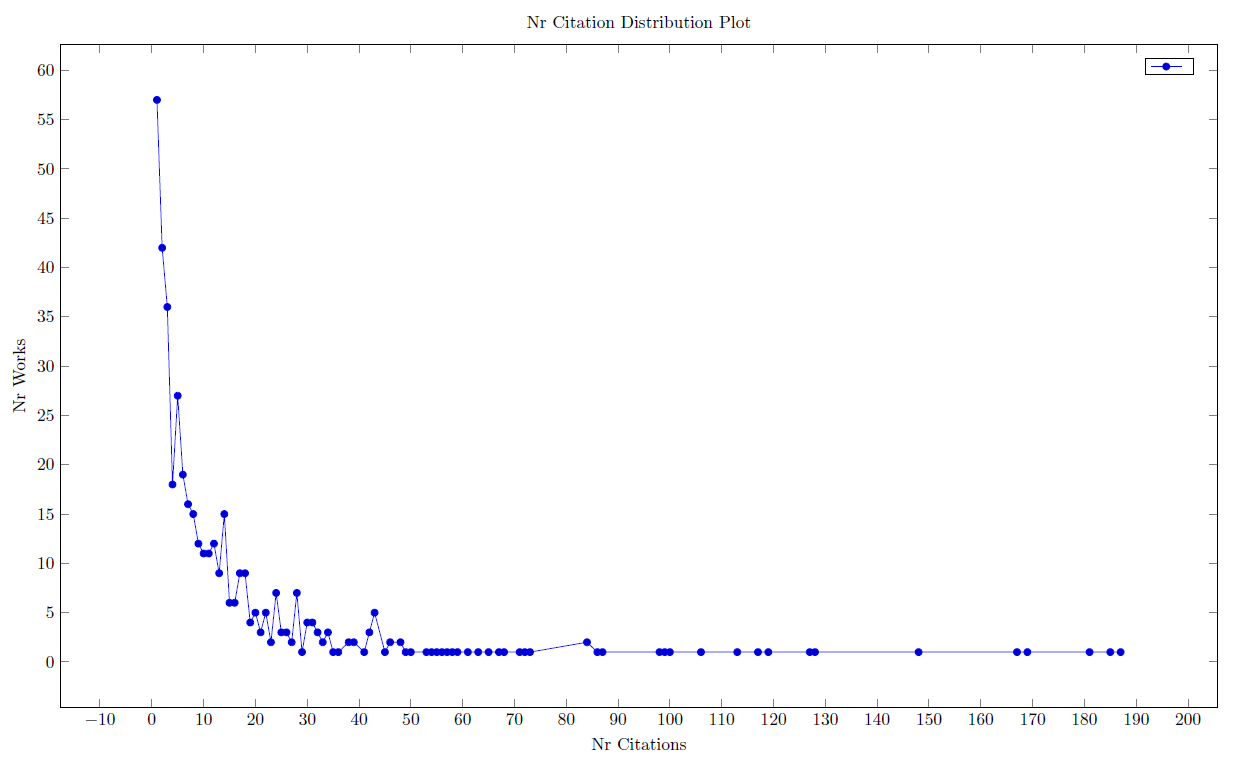
\includegraphics[width=.8\textwidth]{survey/citationcount}
\end{frame}

\begin{frame}
\frametitle{Reuse Example: Survey of Car Sequencing}
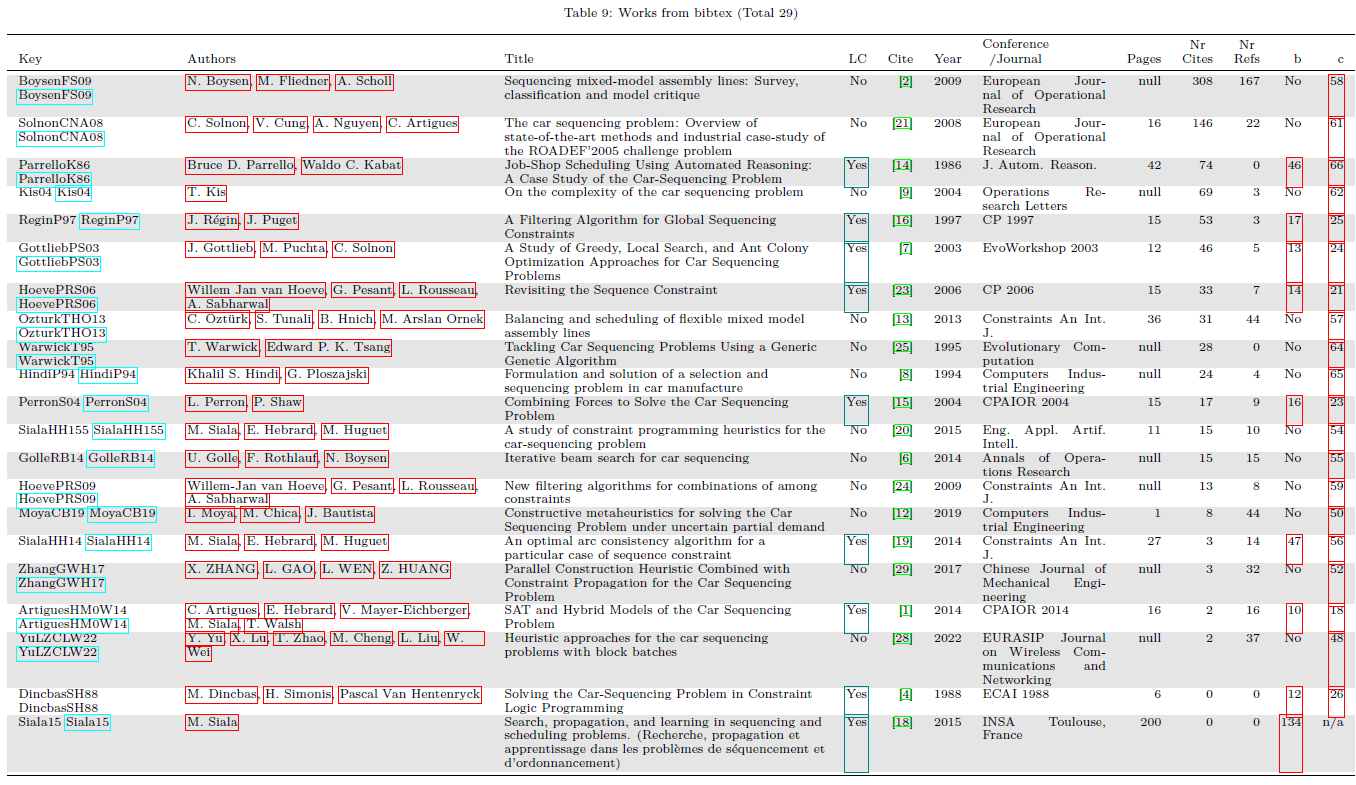
\includegraphics[width=\textwidth]{survey/carsequencing}
\end{frame}


